\begin{boiboiboite}
	\propeau
\end{boiboiboite}

\subsubsection{Température et pression d’ébullition}
\label{exo_temperature_pression_ebullition}

	Un/e étudiant/e voyage à bord d’un avion de ligne et se voit servir une boisson chaude (\cref{fig_cafe}) par l’équipage ; la boisson est presque à ébullition. Il/elle en mesure la température à~\SI{88,2}{\degreeCelsius}.	
	
	\begin{enumerate}
		\item Quelle est la pression dans la cabine ?
	\end{enumerate}
	
	L’avion subit une dépressurisation rapide et la pression de la cabine s’égalise avec la pression atmosphérique locale (\SI{17,2}{\kilo\pascal}). L’étudiant/e enfile son masque à oxygène et constate avec déplaisir que la boisson, qui refroidit, s’est mise à bouillir. 
	
	\begin{enumerate}
	\shift{1}
		\item À quelle température l’ébullition cessera-t-elle ?
	\end{enumerate}
	
	\begin{figure}[htp] %handmade
		\begin{center}
			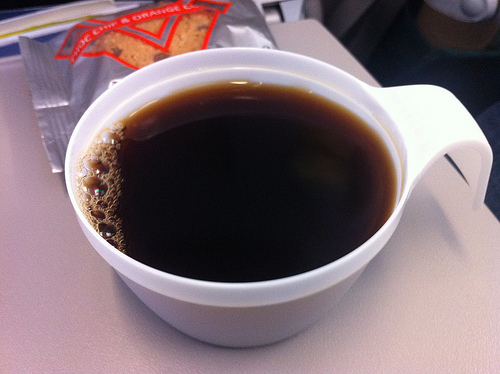
\includegraphics[width=5cm]{images/exercice_cafe.jpg}
		\end{center}
		\supercaption{Boisson chaude aérienne au goût non identifié.}{\href{https://secure.flickr.com/photos/notbrucelee/7942977960/}{photo} \ccby par \flickru{notbrucelee}}
		\label{fig_cafe}
	\end{figure}


\subsubsection{Évaporation d’eau}
\label{exo_evaporation_eau}

	\begin{enumerate}
		\item Combien faut-il de chaleur pour évaporer entièrement une casserole d’eau ? Le récipient contient \SI{2.5}{\liter} d’eau à~\SI{10}{\degreeCelsius}, et la pression atmosphérique ambiante est de~\SI{1}{\bar}. 
		\item Représentez l’évolution sur un diagramme pression-volume, de façon qualitative (c’est-à-dire sans représenter les valeurs numériques), et en y représentant la courbe de saturation.
		\item Le réchauffement est effectué avec une plaque électrique de~\SI{1500}{\watt}. Combien de temps faut-il pour vaporiser l’eau, et quel est le coût engendré par l’expérience ? L’opérateur facture \num{0,15}\euro{} par \si{\kilo\watt\hour} et les pertes de la plaque dans la pièce sont de l’ordre de~\SI{10}{\percent}. 
	\end{enumerate}

	\begin{figure}[htp] %handmade
		\begin{center}
			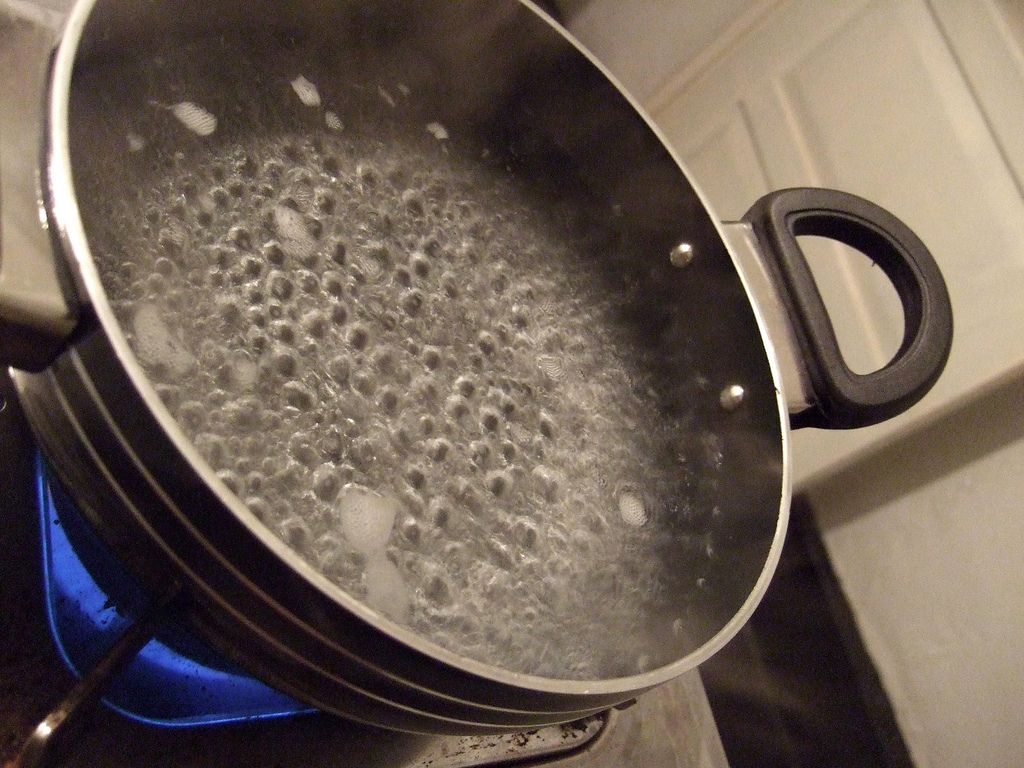
\includegraphics[width=5cm]{images/exercice_boiling.jpg}
		\end{center}
		\supercaption{Expérience de physique ordinaire}{photo \ccby par \flickrun{indi}{Indi Samarajiva}}
	\end{figure}


\subsubsection{Exercice simple de cours}
\label{exo_cours_vapeur_isotherme}
% Cet exo est lié à l’exercice 8.5 (\ref{exo_diagrammes_ts})

	Décrivez très brièvement une expérience permettant de réchauffer à température constante une masse fixe d’eau liquide sous-refroidie. Représentez l’évolution sur un diagramme pression-volume, de façon qualitative, et en y représentant la courbe de saturation.


\subsubsection{Génération de vapeur à haute pression}
\label{exo_generation_vapeur}
% Cet exo est lié à l’exercice 8.5 (\ref{exo_diagrammes_ts})

	Un procédé industriel chimique nécessite l’apport d’un débit de vapeur de~\SI{2}{\kilogram\per\second} à~\SI{6}{\bar} et~\SI{875}{\degreeCelsius}. La machine en charge de fournir cette vapeur est alimentée par une canalisation d’eau liquide pressurisée à~\SI{10}{\degreeCelsius} et~\SI{6}{\bar}.

	\begin{enumerate}
		\item Quelles puissances sous forme de travail et de chaleur sont nécessaires pour générer ce débit ?
		\item Représentez l’évolution subie par l’eau sur un diagramme pression-volume, de façon qualitative et en y représentant la courbe de saturation.
	\end{enumerate}


\subsubsection{Tout est dans le bouchon}
\label{exo_cocotteminute}

	Un/e étudiant/e décide de maintenir une alimentation équilibrée, et fait cuire des aliments dans un autocuiseur (couramment appelé «~cocotte-minute~», \cref{fig_cocotte}). 
		
	La soupape (couramment appelée «~bouchon~») de l’autocuiseur pèse \SI{216}{\gram} ; elle est posée sur un conduit d’échappement de diamètre \SI{5}{\milli\metre}. La pression atmosphérique ambiante est de~\SI{1,1}{\bar}.
	
	\begin{enumerate}
		\item À quelle température l’autocuiseur permet-il de faire cuire les aliments ?
		\item Quelle température et quelle pression une personne appuyant sur la soupape pourrait-elle générer à l’intérieur de l’autocuiseur ? Comment empêcher un accident ?
	\end{enumerate}

	\begin{figure}[htp] %handmade
		\begin{center}
			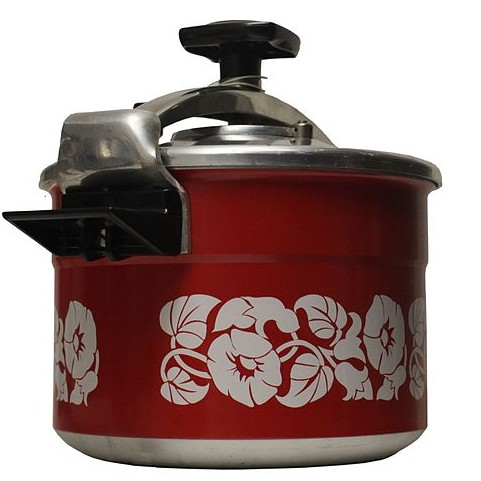
\includegraphics[width=8cm, max width=0.7\columnwidth]{images/exercice_super_cocotte}
		\end{center}
		\supercaption{Autocuiseur ou cuiseur à pression, couramment appelé \textit{«~cocotte-minute~»} en France.}{\wcfile{Super_Cocotte_decor_SEB-MGR_Lyon-IMG_9918.jpg}{Photo} \ccbysa par \wcu{rama}}
		\label{fig_cocotte}
	\end{figure}


\subsubsection{Un premier moteur à vapeur}
\label{exo_moteur_basique_vapeur}

	Un/e ingénieur/e expérimente avec de la vapeur d’eau, dans l’idée de mettre au point un petit moteur très simple (\cref{fig_moteurvapeursimple})
	
	Il/elle insère \SI{2}{\liter} d’eau liquide à~\SI{20}{\degreeCelsius} dans un grand cylindre. L’eau est comprimée à~\SI{2}{\bar} par un piston.
	
	Il/elle chauffe l’eau, et le piston se déplace en maintenant la pression constante, jusqu’à ce que le volume ait atteint~\SI{300}{\liter}.
	
	\begin{enumerate}
		\item Représentez l’évolution sur un diagramme pression-volume, de façon qualitative et en y représentant la courbe de saturation.
		\item Quel a été le travail effectué ?
		\item Combien de chaleur a-t-il fallu apporter ?
		\item Quels seraient les transferts de travail et de chaleur si la détente était poursuivie jusqu’à~\SI{4500}{\liter} ?
	\end{enumerate}

	\begin{figure}[htp] %handmade
		\begin{center}
			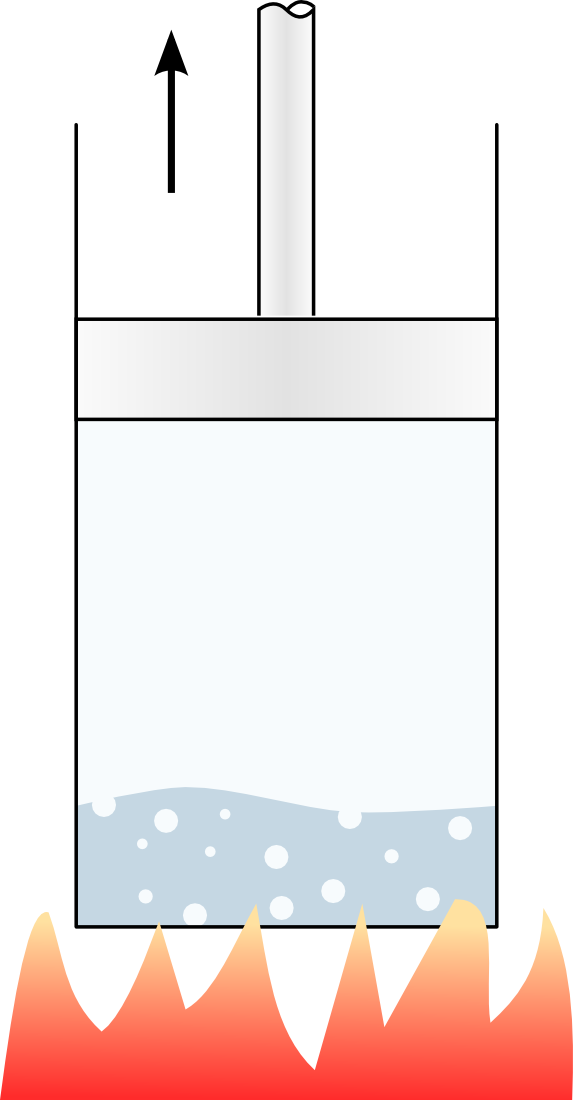
\includegraphics[width=4cm]{images/exercice_moteur_simple.png}
		\end{center}
		\caption{Un concept très simple de moteur à vapeur}
		\label{fig_moteurvapeursimple}
	\end{figure}


\subsubsection{Pompage d’eau}
\label{exo_pompage_baliani}

	Une pompe à liquide est installée pour prélever de l’eau à~\SI{5}{\degreeCelsius} située dans un réservoir en contrebas (\cref{fig_pompage}). 
	
	\begin{enumerate}
		\item Jusqu’à quelle hauteur peut-on effectuer le pompage ?	
		\item Comment pourrait-on procéder pour pomper l’eau à plus grande hauteur ?
	\end{enumerate}

	\begin{figure}[htp] %handmade
		\begin{center}
			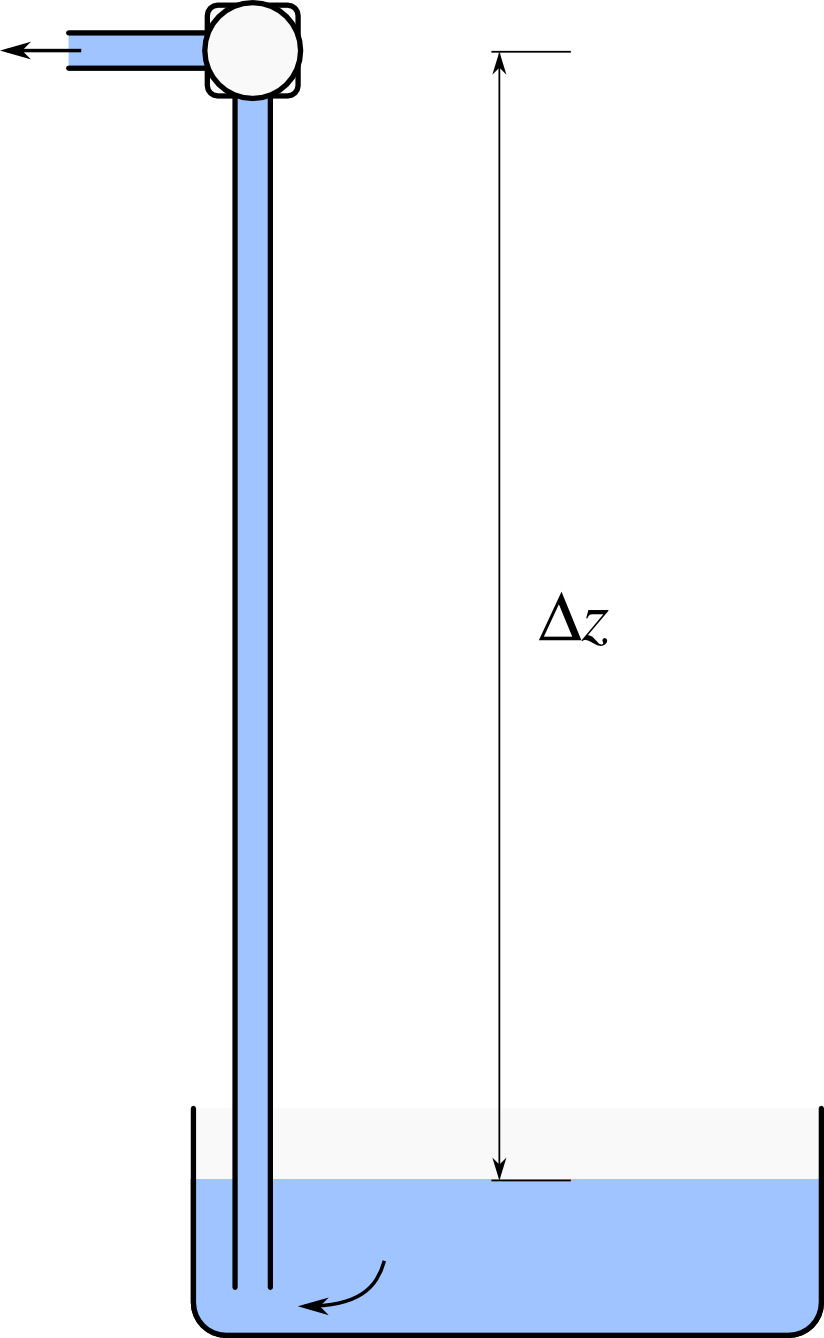
\includegraphics[width=5cm]{images/exercice_pompe_eau.png}
		\end{center}
		\supercaption{Pompage d’un réservoir d’eau situé en contrebas. La première observation de la limite de hauteur calculée dans cet exercice est faite en 1630 par \wf{Giovanni Battista Baliani}.}{\cczero}
		\label{fig_pompage}
	\end{figure}



\subsubsection{Turbine à vapeur sur installation légère}
\label{exo_turbine_vapeur_legere}

	Une entreprise développe une petite centrale à vapeur pouvant être embarquée dans un conteneur de taille standard. Une fois reliée à une chaudière externe, elle est capable de convertir en électricité de la chaleur provenant de combustibles peu raffinés (comme le bois, le papier ou le charbon), avec une efficacité intéressante.
	
	Au sein de cette centrale, la turbine est adiabatique et admet \SI{5}{\tonne\per\hour} de vapeur à~\SI{90}{\bar} et~\SI{510}{\degreeCelsius} en provenance de la chaudière. La pression de sortie est (à peine supérieure à) la pression atmosphérique (nous prendrons \SI{1}{\bar}). Un/e ingénieur prévoit\footnote{Nous pourrons aussi faire cela après le \courshuit.} que l’énergie interne spécifique de la vapeur sera alors de~\SI{2676,6}{\kilo\joule\per\kilogram}.
	
	La turbine est mécaniquement connectée à une génératrice de courant d’efficacité~\SI{85}{\percent}.
	
	\begin{enumerate}
		\item Quelle est la puissance électrique dégagée par la génératrice ?
	\end{enumerate}
	
	À l’autre extrémité du conteneur, une pompe électrique (seul autre élément mécanique de l’installation) récupère l’eau condensée à l’état de liquide saturé (\SI{1}{\bar}) et augmente à nouveau sa pression jusqu’à~\SI{90}{\bar} pour alimenter la chaudière. On considère que lors du pompage, le volume spécifique de l’eau varie de façon négligeable, et que la compression est réversible.
	
	\begin{enumerate}
	\shift{1}
		\item Quelle puissance électrique est prélevée pour alimenter la pompe ?
	\end{enumerate}
	



\subsubsection{Le baril écrasé}
\label{exo_baril}

	Pour effectuer une démonstration de physique, un groupe d’étudiants porte de l’eau à ébullition, à pression ambiante, dans un ancien baril de pétrole (contenance \SI{208}{\liter}, hauteur \SI{88}{\centi\metre}).
	
	Le baril est retiré de la source de chaleur et fermé de façon hermétique. Le but de l’opération est de pouvoir observer le baril se faire écraser par l’atmosphère suite au changement d’état de l’eau qu’il contient.

	\begin{enumerate}
		\item Quelle dépression peut-on générer à l’intérieur du baril en le laissant se refroidir ? 
		\item Quelle serait alors la force verticale s’appliquant sur la paroi supérieure du baril ?
	\end{enumerate}
	
	\textit{Quelques questions plus difficiles :}
		
	\begin{enumerate}
	\shift{2}
		\item Il reste \SI{5}{\liter} de liquide au fond du baril à la fermeture du bouchon. Quel est le titre de la vapeur ?
		\item Quelle masse de vapeur s’est condensée pendant le refroidissement ?
		\item Combien a-t-il fallu retirer de chaleur pour atteindre la dépression finale ?
	\end{enumerate}

%\clearpage %handmade
\subsubsection{Moteur Newcomen}
\label{exo_moteur_newcomen}

	À leur époque, autour de 1720, les moteurs Newcomen (\cref{fig_newcomen}) étaient à la pointe de la technologie. On insérait dans un grand cylindre (hauteur \SI{1}{\metre}, diamètre \SI{1.5}{\metre}) de la vapeur à peine surchauffée (\SI{1}{\bar}, \SI{250}{\degreeCelsius}).
	
	Puis, on refroidissait cette vapeur (en laissant entrer une faible quantité d’eau liquide à pression et température atmosphériques), en maintenant la pression interne à~\SI{0,1}{\bar}. Le piston redescendait ainsi en fournissant du travail.
	
	L’eau disponible pour alimenter le moteur est à~\SI{1}{\bar}, \SI{10}{\degreeCelsius}.
	
	\begin{enumerate}
		\item Tracez l’évolution suivie par l’eau sur un diagramme pression-volume ou température-volume, en y indiquant la courbe de saturation.
		\item Avant de pouvoir effectuer la descente, quelle quantité de chaleur faut-il fournir pour remplir le cylindre de vapeur ?
		\item Quelle quantité de travail est dégagée par le moteur pendant la descente du piston ?\\
				\textit{Indice : il faut tenir compte du travail effectué par l’atmosphère sur la face extérieure du piston.}
		\item Quel est ainsi le rendement du moteur, si l’on néglige les frottements et toutes les autres pertes de chaleur ?
	\end{enumerate}

	\begin{figure}
		\begin{center}
			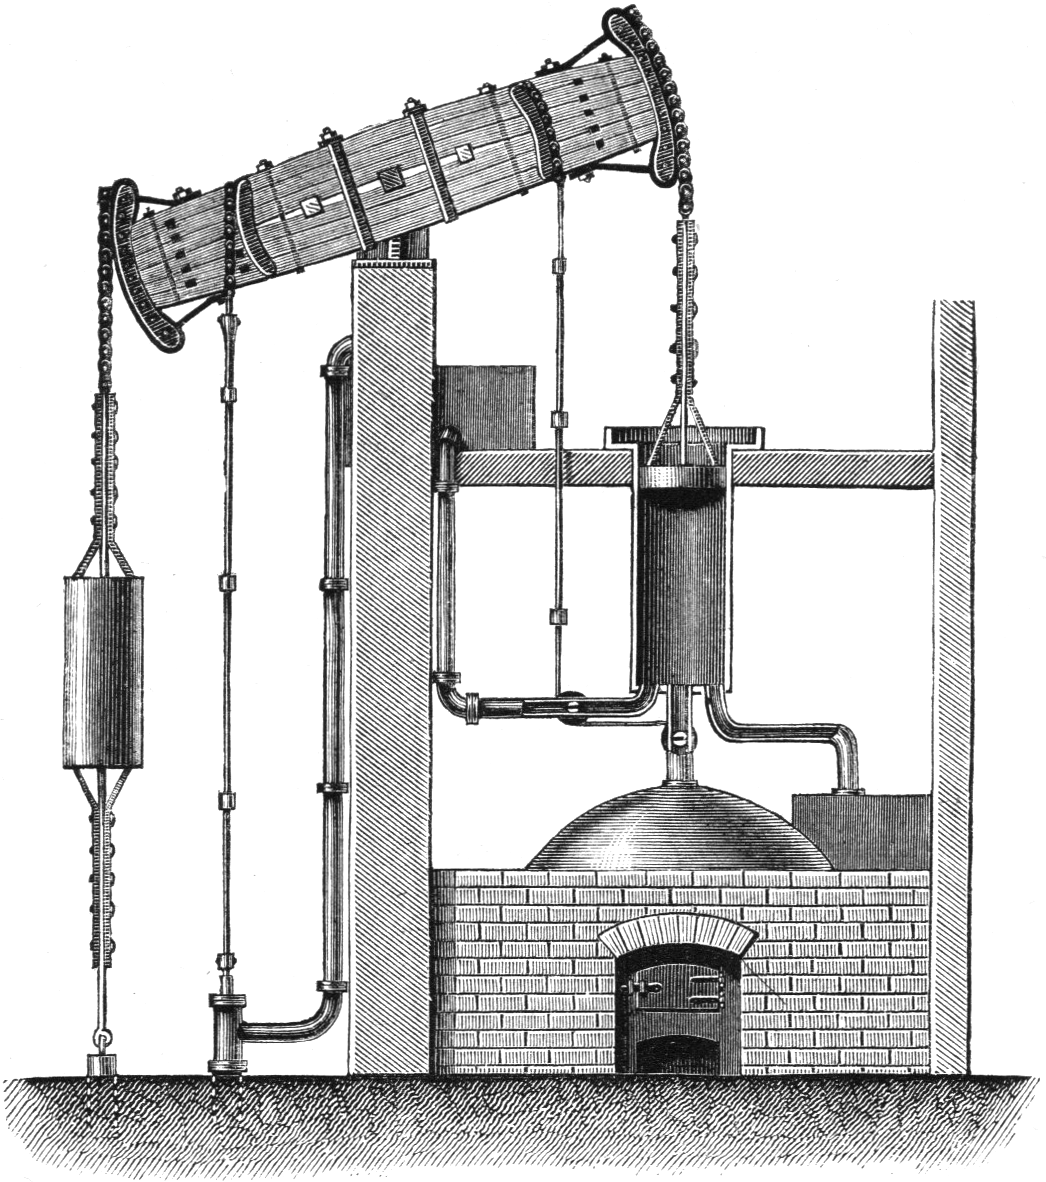
\includegraphics[width=9cm]{images/moteur_newcomen_2.png}
		\end{center}
		\supercaption{L’ingénieux moteur atmosphérique de Newcomen, premier véritable succès de la motorisation vapeur.}{\wcfile{GesNat662.jpg}{schéma} \pd C. L. Moll -- \textit{Die gesammten Naturwissenschaften} (1873)}
		\label{fig_moteur_newcomen}
	\end{figure}



\subsubsection{Condenseur de centrale à vapeur}
\label{exo_condenseur_riviere}

	Dans une centrale électrique de grande puissance, le condenseur est en charge de récupérer l’eau à la sortie des turbines, et de lui retirer de l’énergie pour qu’elle puisse retourner à l’état liquide et ré-intégrer le circuit pompes $\to$ chaudières $\to$ turbines. L’eau du circuit (\SI{180}{\tonne\per\hour}) arrive à~\SI{0,5}{\bar} avec un volume spécifique de~\SI{3,1247}{\metre\cubed\per\kilogram} ; elle doit repartir à la même pression, à l’état de liquide saturé.
	
	Pour extraire de la chaleur à l’eau de la centrale, les condenseurs utilisent un circuit d’eau secondaire provenant directement d’une rivière. On y prélève de l’eau à~\SI{10}{\degreeCelsius}.
	
	Pour réduire l’impact écologique de la centrale, on souhaite rejeter l’eau secondaire dans la rivière à une température égale ou inférieure à~\SI{35}{\degreeCelsius}.
	
	\begin{enumerate}
		\item Quel débit d’eau secondaire doit-on prélever en rivière ?
		\item Pour limiter les rejets de chaleur en rivière, où (et comment) rejette-t-on aussi, en pratique, la chaleur du condenseur ?
	\end{enumerate}
	

\subsubsection{Catapulte de porte-avions}
\label{exo_catapulte}

	Une catapulte à avions est montée sur un navire militaire (figures \ref{fig_exo_catapulte_1} et \ref{fig_exo_catapulte_2}). Elle est constituée d’un réservoir de vapeur connecté à un long cylindre, dans lequel glisse un piston entraînant l’avion au décollage.
	
	Au début du catapultage, la vapeur est à~\SI{140}{\bar} et~\SI{700}{\degreeCelsius}. Après une brève course de~\SI{50}{\metre}, l’avion a quitté le pont et la vapeur est à~\SI{4}{\bar} et~\SI{410}{\degreeCelsius}.
	
	\begin{enumerate}
		\item Quelle énergie la catapulte a-t-elle fourni à l’avion par kilo de vapeur ?
		\item Quelles doivent être le diamètre du piston, et la masse totale de vapeur, pour que la poussée fournie à l’avion soit toujours supérieure à~\SI{2,5}{\tonne} ?
	\end{enumerate}
	
	\textit{Et une question à laquelle nous ne savons pas encore répondre :} Quelle est la quantité \emph{maximale} d’énergie que la catapulte aurait pu fournir à l’avion en laissant la vapeur se détendre ?
	
	\begin{figure}
		\begin{center}
			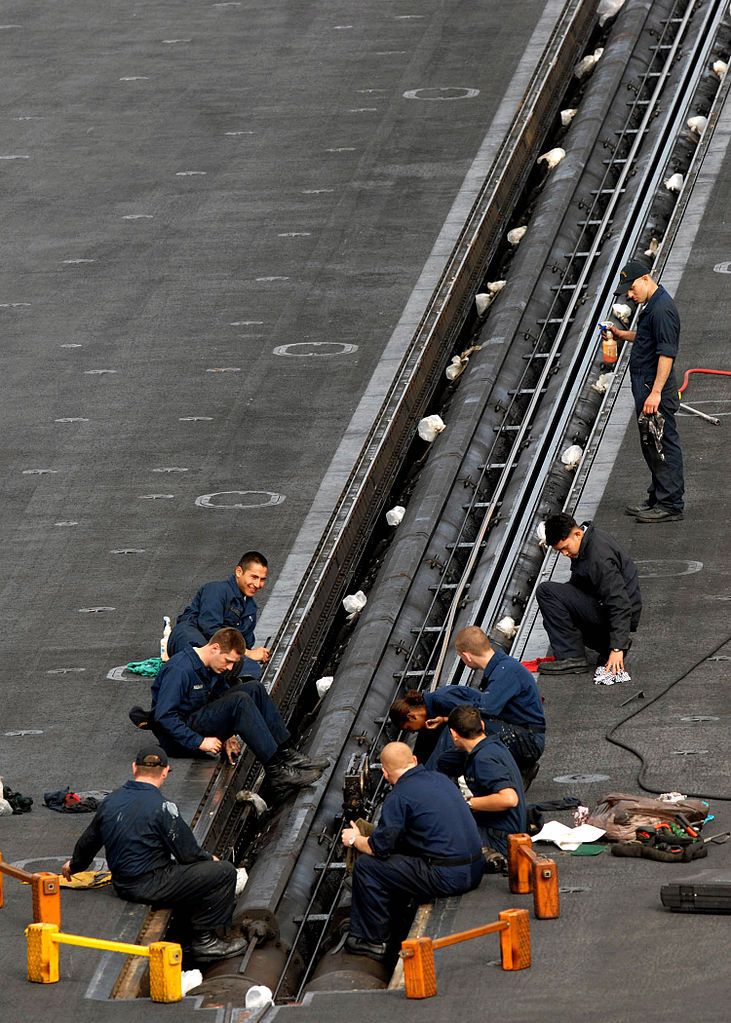
\includegraphics[width=0.8\columnwidth]{images/catapulte_vapeur_1.jpg}
		\end{center}
		\supercaption{Cylindre d’une catapulte à vapeur du USS Abraham Lincoln}{\wcfile{Catapulte CVN72 071117-N-9898L-006.jpg}{Photo} \pd par Geoffrey Lewis, U.S. Navy}
		\label{fig_exo_catapulte_1}
	\end{figure}
	\begin{figure}
		\begin{center}
			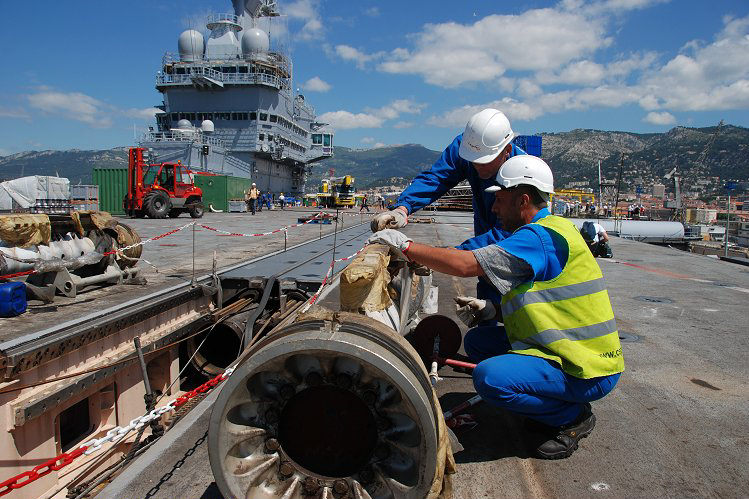
\includegraphics[width=\columnwidth]{images/catapulte_vapeur_2.jpg}
		\end{center}
		\supercaption{Piston d’une catapulte à vapeur du Charles de Gaulle (droite).}{\wcfile{French aircraft carrier Charles de Gaulle - catapult maintenance 2008.jpg}{Photo} \ccbysa par Jean-Michel Roche, Netmarine.net}
		\label{fig_exo_catapulte_2}
	\end{figure}


\subsubsection{Turbine de centrale nucléaire}
\label{exo_turbine_balakovo}

	Dans une centrale nucléaire, la génératrice d’électricité est entraînée par une turbine à vapeur (\cref{fig_centrale_balakovo}).\\
	La majorité de la vapeur (chauffée par le réacteur nucléaire) traverse l’entièreté de la turbine. Toutefois, au milieu de la turbine, on procède à un prélèvement de vapeur. Il permet, d’une part, de réchauffer l’eau d’une autre partie du circuit (\S\ref{ch_regeneration}), et d’autre part, de contrôler précisément le débit de masse en circulation. Le débit total à l’entrée est de~\SI{317}{\tonne\per\hour} de vapeur.
	
	On mesure les propriétés de vapeur suivantes :
	
	\begin{description}
	\TabPositions{0.3\columnwidth} %handmade, pour faire tenir les données
		\item Entrée : 		\tab\SI{120}{\bar} ; 	\SI{565}{\degreeCelsius}
		\item Prélèvement : 	\tab\SI{10}{\bar} ; 	\SI{250}{\degreeCelsius} ;	\SI{1,2}{\kilogram\per\second}
		\item Sortie : 		\tab\SI{1}{\bar} ;		\SI{115}{\degreeCelsius}
	\end{description}

	Quelle est la puissance mécanique fournie par la turbine ?

	\begin{figure}
		\begin{center}
			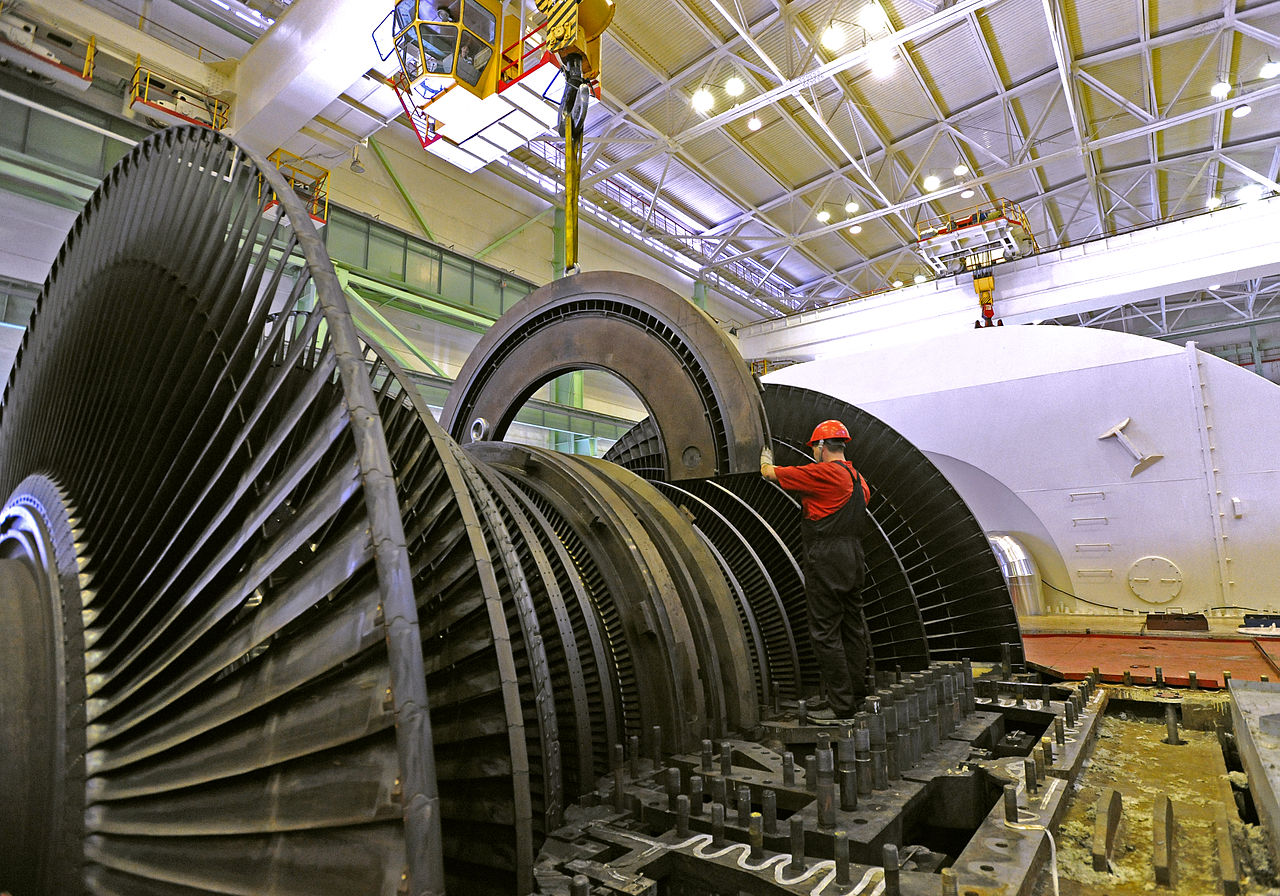
\includegraphics[height=0.33\textwidth]{images/exercice_turbine_centrale2.jpg}
			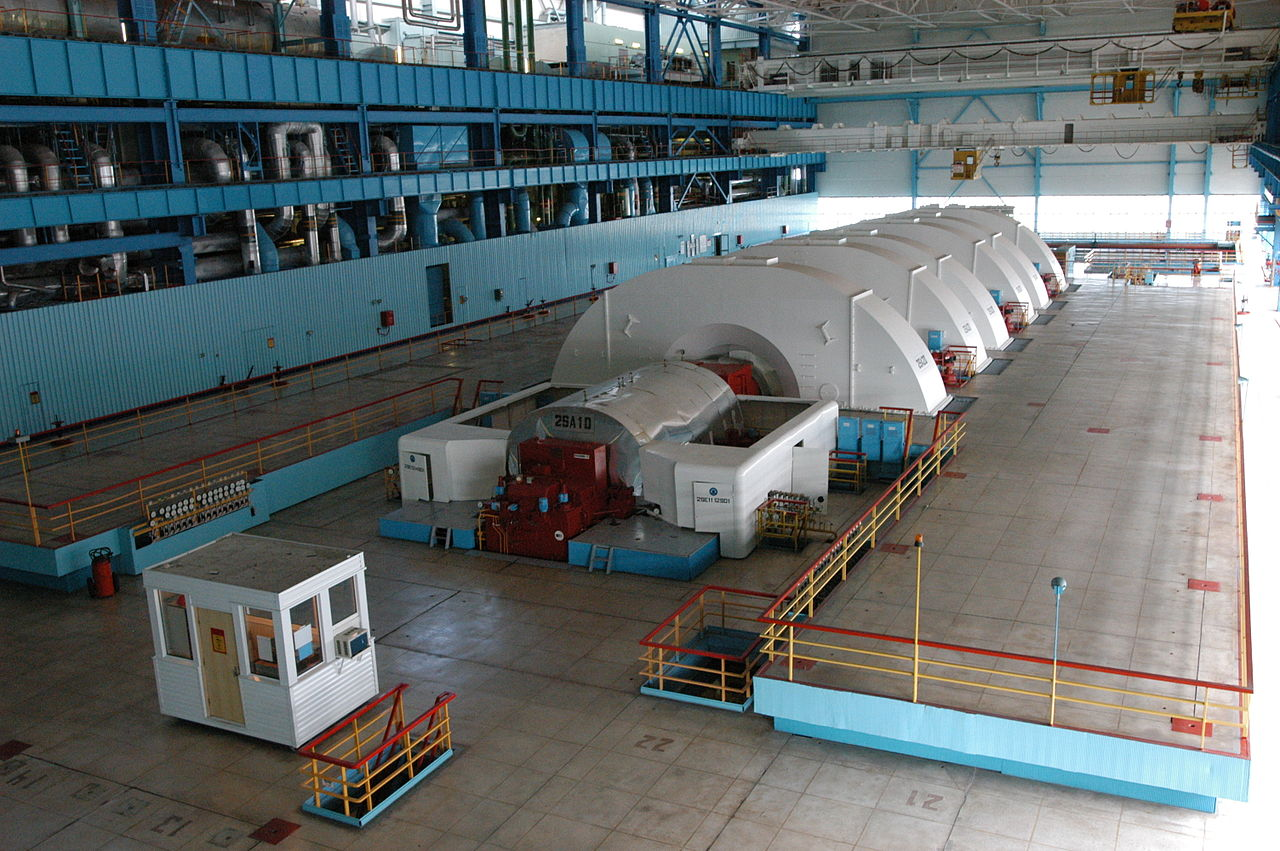
\includegraphics[height=0.33\textwidth]{images/exercice_turbine_centrale1.jpg}
		\end{center}
		\supercaption{Une des turbines de la centrale nucléaire russe de Balakovo (puissance centrale approx.~\SI{1}{\giga\watt}), en maintenance (haut) et en installation (bas).}{\wcfile{BalakovoNPP_turb.JPG}{photo 1} et \wcfile{BalNPP_m_st2.jpg}{2} \ccbysa The Centre of the Public Information Balakovo NPP}
		\label{fig_centrale_balakovo}
	\end{figure}

\exercisesolutionpage
\titreresultats

\begin{description}
	\item [\ref{exo_temperature_pression_ebullition}] 
			\tab 1) Par interpolation entre $T_\text{sat} = \SI{85}{\degreeCelsius}$ et $T_\text{sat} = \SI{90}{\degreeCelsius}$ dans l’abaque n°2, on obtient $p_\text{sat} = \SI{0,67}{\bar}$
			\tab 2) Par interpolation entre $p_\text{sat} = \SI{0,016}{\mega\pascal}$ et $p_\text{sat} = \SI{0,018}{\mega\pascal}$ dans l’abaque n°3, on obtient $T_\text{sat} = \SI{56,8}{\degreeCelsius}$ (berk!)
	\item [\ref{exo_evaporation_eau}]
			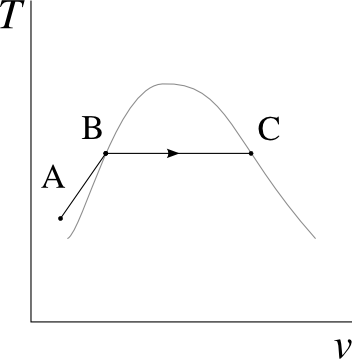
\includegraphics[width=\solutiondiagramwidth]{images/exo_sol_tv_ebullition.png}
			\tab 1) Pour chauffer l’eau jusqu’à ébullition (B) puis évaporation totale (C) : $Q_{\A \to \C} = m (q_\fromatob + q_\frombtoc) = \frac{V_\A}{v_\A}(h_{L \SI{0,1}{\mega\pascal}} - h_\A + h_{LV \SI{0,1}{\mega\pascal}}) = \SI{+6582}{\kilo\joule}$. 
			\tab 3) $\Delta t = \frac{Q_{\A \to \C}}{\dot Q_\text{moyenne}} = \SI{1}{\hour} ~\SI{21}{\minute}$ pour un coût effarant de \num{0,29}\euro{}.
	\item [\ref{exo_cours_vapeur_isotherme}]
			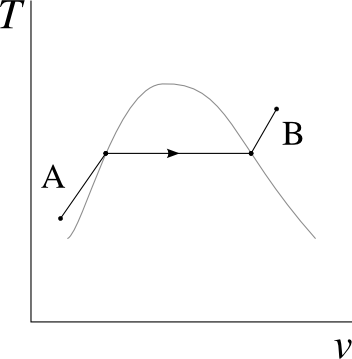
\includegraphics[width=\solutiondiagramwidth]{images/exo_sol_tv_generation_vapeur.png}
			\tab cf. \S\ref{ch_lv_bain_marie} \& \cref{fig_p-v_eau}.
	\item [\ref{exo_generation_vapeur}] 
			\tab 1) Par lecture dans l’abaque n°1 @ $p_\A = \SI{0,6}{\mega\pascal}$, $h_\A = \SI{42,6}{\kilo\joule\per\kilogram}$. En interpolant entre \num{800} et \SI{900}{\degreeCelsius} dans cette même table, on obtient $h_\B = \SI{4336,6}{\kilo\joule\per\kilogram}$. Ainsi avec l’\cref{eq_lv_chaleur_isobare} (, $\dot{Q}_\fromatob = \dot m \Delta h = \SI{+8,59}{\mega\watt}$. $\dot{W}\fromatob = \SI{0}{\watt}$ (\ref{eq_lv_travail_isobare}).
	\item [\ref{exo_cocotteminute}] 
			\tab 1) $p_\text{intérieur} = p_\text{bouchon} + p_\text{atm.} = \frac{F_\text{poids}}{S_\text{bouche}} + \SI{1}{\bar} = \SI{2,0797}{\bar}$. Par interpolation dans l’abaque n°2, $T_{\text{sat.} p=\SI{2,0797}{\bar}} = \SI{121,37}{\degreeCelsius}$.
	\item [\ref{exo_moteur_basique_vapeur}]
			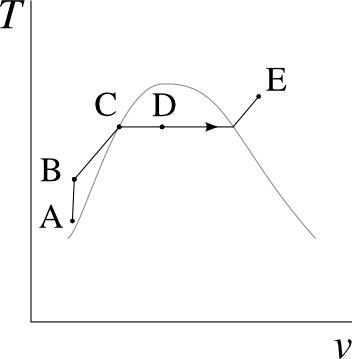
\includegraphics[width=\solutiondiagramwidth]{images/exo_sol_tv_moteur_basique_1.png}
			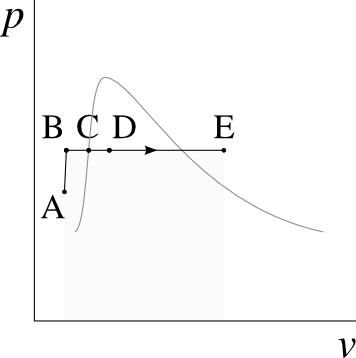
\includegraphics[width=\solutiondiagramwidth]{images/exo_sol_pv_moteur_basique_2.png}
			\tab 2) $W_\fromatob \approx 0$ (\ref{eq_lv_sf_travail_isochore}) ; avec $m = \frac{V_\B}{v_\B}$ et $v_\D = \frac{V_\D}{m}$, on calcule $W_{\B \to \D} = - m p_\text{cste.} (v_\D - v_\B) = \SI{-59,6}{\kilo\joule}$ (\ref{eq_lv_sf_travail_isobare}).
			\tab 3) Avec $v_\D$ on calcule le titre $x_\D \approx \frac{v_\D}{v_{V \SI{0,2}{\mega\pascal}}} = \num{0,1697}$. 
				Ainsi, ${Q}_{\B \to \D} = m (h_\D - h_\B) = m (h_L + x_\D h_{LV} - h_\B) = \SI{+1585,2}{\kilo\joule}$ (\ref{eq_lv_sf_chaleur_isobare}), soit vingt-cinq fois plus…
			\tab 4) Les relations sont identiques et donnent ${W}_{\B \to \E} = \SI{-899,6}{\kilo\joule}$ et ${Q}_{\B \to \E} = \SI{+7694,3}{\kilo\joule}$ (le rendement saute de \num{3,8} à \SI{11,7}{\percent}… il y a là une piste à suivre…)
	\item [\ref{exo_pompage_baliani}] 
			\tab 1) La pression hydrostatique dans la canalisation dépend de la hauteur ($\Delta p = \rho g \Delta z$). Lorsque la pression à la pompe chute sous $p_\text{sat.}$, l’eau se met à bouillir. Pour $\Delta p_\text{ébullition} = \SI{9,9127e4}{\pascal}$, $\Delta z_\text{ébullition} = \SI{10,1}{\metre}$. 
			\tab 2) Il y a mieux que de réchauffer le réservoir…
	\item [\ref{exo_turbine_vapeur_legere}] 
			\tab 1) En A dans l’abaque n°1 nous interpolons à \SI{9}{\mega\pascal} entre \num{500} et \SI{600}{\degreeCelsius} pour obtenir $h_{\SI{510}{\degreeCelsius} \& \SI{90}{\bar}} = \SI{3412}{\kilo\joule\per\kilogram}$. 
				Idem en B où $u_\B > u_{V \SI{1}{\bar}}$ ($h_\B = \SI{2899,4}{\kilo\joule\per\kilogram}$). 
				Enfin $\dot{W}_\text{électrique} = \eta_\text{conversion} \dot m \Delta h = \SI{-605,8}{\kilo\watt}$.
			\tab 2) $\dot{W}_\text{pompe} = \dot m \int v \diff p \approx \dot m v_L \Delta p = \SI{+12,9}{\kilo\watt}$.
	\item [\ref{exo_baril}] 
			\tab 1) Si on atteint $T_\B = \SI{30}{\degreeCelsius}$ à volume constant, alors $p_\text{intérieur min.} = p_{\text{sat.} \SI{30}{\degreeCelsius}} = \SI{0,004247}{\mega\pascal}$. Alors  $\Delta p_\text{max} = \SI{-9,575e4}{\pascal}$ ;
					\tab\tab 2) $F_\text{max} = \Delta p_\text{max} S_\text{couvercle} = \SI{22,6}{\kilo\newton}$ (le baril sera bien sûr écrasé avant)
					\tab 3) $x_\A = \num{0,02408}$, $x_\B = \num{7,328e-4}$ ;
					\tab 4) $m_\text{condensée} = \SI{4,9138}{\kilogram}$ ;
					\tab 5) ${Q}_\fromatob = \SI{-1,878}{\mega\joule}$.
	\item [\ref{exo_moteur_newcomen}]
			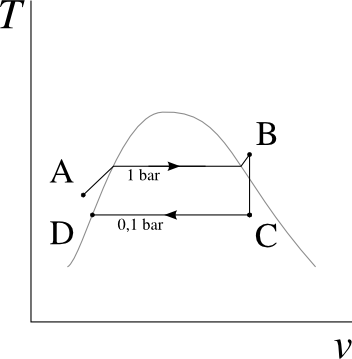
\includegraphics[width=\solutiondiagramwidth]{images/exo_sol_tv_newcomen.png} 
			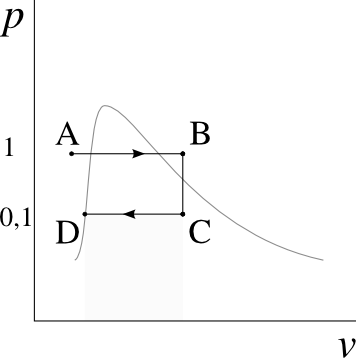
\includegraphics[width=\solutiondiagramwidth]{images/exo_sol_pv_newcomen.png}
			\tab 2) Une lecture de l’abaque n°1 donne $h_\A = \SI{42,1}{\kilo\joule\per\kilogram}$. Par interpolation nous obtenons $h_\B = \SI{2975}{\kilo\joule\per\kilogram}$ et $m = \frac{V_\B}{v_\B} = \SI{0,7354}{\kilogram}$. Ainsi nous calculons ${Q}_\fromatob = m \Delta h = \SI{+2154}{\kilo\joule}$ (\ref{eq_lv_sf_chaleur_isobare}).
			\tab 3) Dans le même tableau que $h_\B$ nous avons déjà obtenu $v_\B = \SI{2,406}{\metre\cubed\per\kilogram}$. Ainsi ${W}_{\text{piston} \to \text{arbre}} = W_{\text{atm.} \to \text{piston}} + W_{\text{piston} \to \text{vapeur}} = m (p_\C - p_\text{ext.}) (v_\D - v_\C) = \SI{-159}{\kilo\joule}$.
			\tab 4) $\eta \equiv \frac{Q_\text{fournie}}{W_\text{utile}} = \SI{7,38}{\percent}$ (valeur réaliste).
	\item [\ref{exo_condenseur_riviere}] 
			\tab 1) $x_\A = \SI{96,44}{\percent}$ \& $x_\B = 0$ ; ainsi $\dot Q_\fromatob = \SI{-111,13}{\mega\watt}$, ce pourquoi il nous faut $\dot{m}_\text{secondaire} \geq \SI{1062,4}{\kilogram\per\second}$.
			\tab 2) Dans l’atmosphère, au moyen de l’eau secondaire rejetée par les larges cheminées…
	\item [\ref{exo_catapulte}] 
			\tab 1) $\Delta u = \SI{-433,1}{\kilo\joule\per\kilogram}$ ($=w_\fromatob$ si l’on suppose l’évolution adiabatique) ;
			\tab 2) $D_\text{min.} = \SI{32,26}{\centi\metre}$ (attention à tenir compte de la pression atmosphérique) ; $m = \frac{V_\text{max} - V_\text{min}}{v_\text{max} - v_\text{min}} = \SI{5,243}{\kilogram}$.
			\tab NB : faute de sources fiables, les données de cet exercice sont purement imaginaires.
	\item [\ref{exo_turbine_balakovo}] \tab $\dot{W}_\text{turbine} = \SI{-71}{\mega\watt}$.
\end{description}
